\chapter{Getting Started in BASIC}
\label{cha:basic-getting-started}

It is possible to code on the MEGA65 in many languages,
however most people start with BASIC.  That makes sense,
because BASIC stands for Beginner's All-purpose Symbolic
Instruction Code: It was made for people like you to get
started with in the world of coding!

A few short words before we dive in: BASIC is a programming
language, and like spoken language it has conventions, grammar
and vocabulary.  Fortunately, it is much quicker and easier
to learn than our complex human languages. But if you pay
attention, you might notice some of these structures, and that
can help you along your path in the world of coding.

If you haven't already read Chapter \ref{cha:getting-started},
it might be a good idea to do so. This will help you be able to
more confidently interact with the MEGA65 computer.

It's also great to remember that if you really confuse the MEGA65,
you can always get back to the READY. prompt by just pressing the
reset button on the left-hand side of the keyboard, or if that
doesn't help, then by turning it off
and on again using the power switch on the left-hand side of the keyboard.
You don't have to worry about shutting the computer
down properly or any of that nonsense.  The only thing to remember
is that if you had any unsaved work, it will be lost when you turn
the computer off and on again or press the reset button.

Finally, if you don't understand all of the descriptions and information
with an example -- don't worry! We have provided as much information
as we can, so that it is there in case you have questions, encounter problems are are
just curious to discover more.  Feel free to skip ahead to the examples
and try thing out, and then you can go back and re-read it when you are motivated
to find something out, or help you work though a problem.  And if you don't find
the answer to your problem, send us a message!  There are support forums for the
MEGA65 at \url{https://mega65.net}, and you can
report problems with this guide at:

\url{https://github.com/mega65/mega65-user-guide}

We hope you have as much fun learning to programme the MEGA65 as
we have had making it!

\section{Your first BASIC programmes}

The MEGA65 was designed to be programmed! When you turn it on,
it takes a couple of seconds to get its house in order, and then
it quickly shows you a ``READY.'' prompt and flashing block called
the cursor.  When the cursor is blinking, it tells you that the
computer is waiting for input.  The ``READY.'' message tells you
that the BASIC programming language is running and ready for you to
start programming.  You don't even need to load any programmes --
you can just get started.

Try typing the following into the computer and see what happens:

\begin{tcolorbox}[colback=black,coltext=white]
\verbatimfont{\codefont}
\begin{verbatim}
HELLO COMPUTER
\end{verbatim}
\end{tcolorbox}

To do this, just type the letters as you see them above.  The computer
will already be in upper-case mode, so you don't need to hold the \specialkey{SHIFT}
or \specialkey{CAPS\\LOCK}} key down.  When you have typed ``HELLO COMPUTER'' press
  the \specialkey{RETURN} key.  This tells the computer you want it to accept the
  line of input you have typed.  When you do this, you should see a message something
  like the following:

  If you saw a \screentext{SYNTAX ERROR} message something like that one, then congratulations:
  You have succeeded in communicating with the computer!\index{Errors!Syntax}\index{SYNTAX ERROR}
  Error messages sound much nastier than they are.  The MEGA65 uses them, especially
  the syntax error to tell you when it is having trouble understanding what you have
  typed, or what you have put in a programme.  They are nothing to be afraid of, and
  experienced programmers get them all the time.

  In this case, the computer was confused because it doesn't understand the word
  ``hello'' or the word ``computer''.  That is, it didn't know what you wanted it to
  do.  In this regard, computers are quite stupid. They know only a few words, and
  aren't particularly imaginative about how the interpret them.

  So let's try that again in a way that the computer will understand.  Try typing
  the following in.  You can just type it right away. It doesn't matter that the
  syntax error message can still be seen on the screen.  The compute has already
  forgotten about that by the time it told you \screentext{READY.} again.

\begin{tcolorbox}[colback=black,coltext=white]
\verbatimfont{\codefont}
\begin{verbatim}
PRINT "HELLO COMPUTER"
\end{verbatim}
\end{tcolorbox}

Again, make sure you don't use shift or shift-lock while typing it in.  The symbols around
the words \screentext{HELLO COMPUTER} are double-quotes.  If you are used to an Australian or American
keyboard, you might discover that they double-quote key is in a rather different place to
where you are used to:  Double-quotes can be typed on the MEGA65 by holding down the
\specialkey{SHIFT} key, and then pressing 2.  Don't forget to press the \specialkey{RETURN}
key when you are done, so that the computer knows you want it to do something with your input.

If you make a mistake while typing, you can use the \specialkey{INST\\DEL} to rub out the mistake
and fix it up.  You can also use the cursor keys to move back and forth on the line while
you edit the line you are typing, but there is a bit of a trick if you have already typed
a double-quote: If you try to use the cursor keys, it will print a funny reversed symbol
instead of moving the cursor.  This is because the computer thinks you want to record
moving the cursor in the text itself, which can be really useful and fun, and which you can
read more about in Chapter \ref{cha:getting-started}. But for now, if you
make a mistake just press the \specialkey{RETURN} key and type the messed up line again.
Hopefully now you will see something like the following:

\setlength{\intextsep}{0pt}%
  \begin{wrapfigure}{i}{0.6\linewidth}
    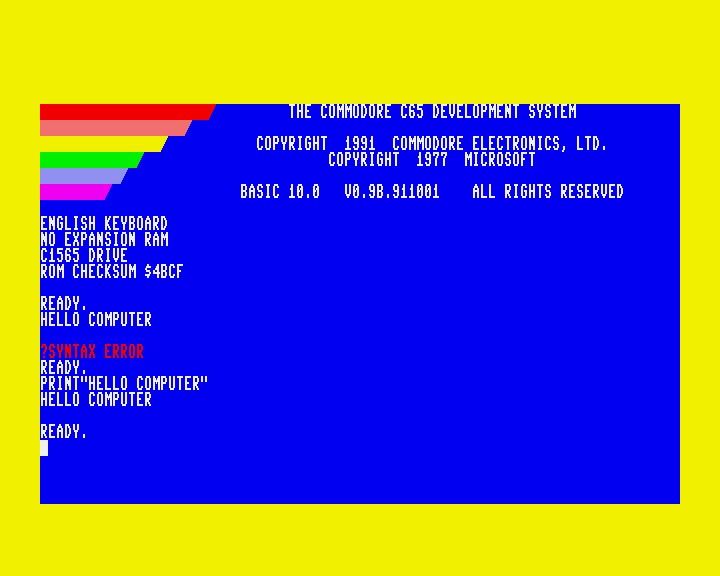
\includegraphics[width=\linewidth]{images/print-hello-computer.png}
  \end{wrapfigure}

  This time no new \screentext{SYNTAX ERROR} message should appear. But if some kind
  of error message has appeared, just try typing in the command again, after
  taking a close look to work out where the mistake might be.

  Instead of an error, we should see \screentext{HELLO COMPUTER} repeated underneath
  the line you typed in.  The reason this happened is that the computer
  does understand the word \screentext{PRINT}.  It knows that whatever comes after
  the word \screentext{PRINT} should be printed to the screen.  We had to put \screentext{HELLO
  COMPUTER} inside double-quotes to tell the compute that we want it to be
  printed literally.

  If we hadn't put the double-quotes in, the computer would have thought
  that \screentext{HELLO COMPUTER} was the name of a stored piece of information.
  You can try it, if you like.

  \begin{wrapfigure}{i}{0.6\linewidth}
    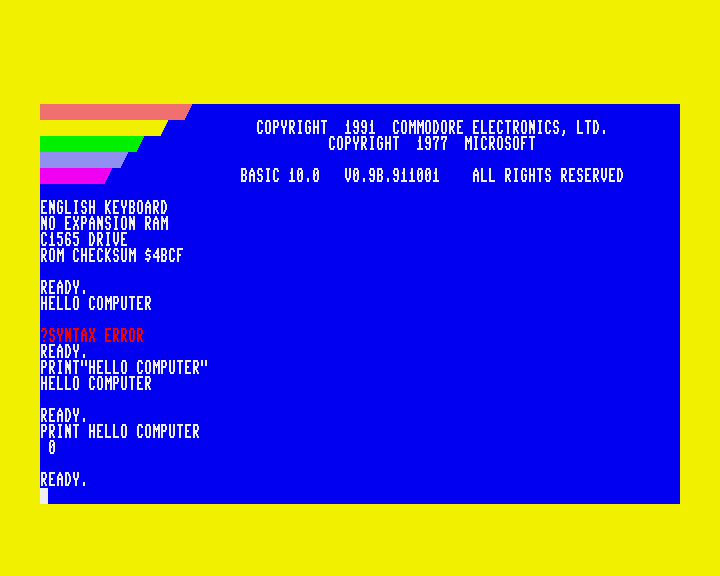
\includegraphics[width=\linewidth]{images/print-hello-computer-no-quotes.png}
  \end{wrapfigure}  

  But because we haven't stored any piece of information in such a place,
  the computer will have zero there, so the computer will print the number
  zero, like this. If the computer prints zero or some other number when
  you expected a message of some sort, this can be the reason.

  In the above examples we typed commands in directly, and the computer executed
  them immediately after you pressed the \specialkey{RETURN} key.  This is why
  typing commands in this way is often called {\em direct mode} or {\em immediate mode}.
  
  But we can also tell the computer to remember a list of commands to execute one
  after the other.   This is done using the rather unimaginatively named {\em non-direct mode}.
  To use non-direct mode, we just put a number between 0 and 63999 at the start of
  the command.  The computer will then remember that command.  Unlike when we executed
  a direct-mode command, the computer doesn't print \screentext{READY.} again. Instead the cursor
  just reappears on the next line, ready for us to type in more commands.

  Let's try that out with a simple little programme.  Type in the following three lines of
  input:

\begin{tcolorbox}[colback=black,coltext=white]
\verbatimfont{\codefont}
\begin{verbatim}
1 FOR I = 1 TO 10 STEP 1
2 PRINT I
3 NEXT I
\end{verbatim}
\index{FOR}
\index{BASIC 10 Commands!FOR}
\end{tcolorbox}

When you have done this, the screen should show something like this:

\setlength{\intextsep}{0pt}%
  \begin{wrapfigure}{i}{0.6\linewidth}
    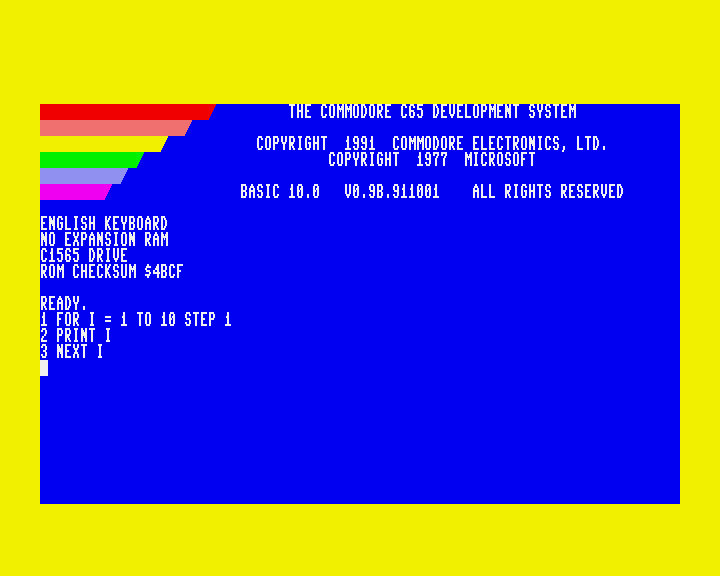
\includegraphics[width=\linewidth]{images/first-steps-for-loop-programme-1.png}
  \end{wrapfigure}

If it doesn't you
can try again. Don't forget, if you feel that the computer is getting all muddled up,
you can just press the reset button or flip the power switch off and on on the left side of the
computer to reboot it. This only takes a couple of seconds, and doesn't hurt the MEGA65
in anyway.

We have told the computer to remember three commands, that is, \screentext{FOR I = 1 TO 10 STEP 1},
\screentext{PRINT I}
and \screentext{NEXT I}.  We have also told the computer which order we would like to run them in: The
computer will start with the command with the lowest number, and execute each command that
has the next higher number in turn, until it reaches the end of the list.  So it's a bit like
a reminder list for the computer. This is what we call a programme, a bit like the programme at
a concert or the theatre, it tells us what is coming up, and in what order.
So let's tell the computer to execute this programme.

But first, let's try to guess what will happen.  Let's start with the middle command, \screentext{PRINT I}.
We've seen the \screentext{PRINT} command, and we know it tells the computer to print things to the screen.
The thing it will try to print is \screentext{I}.  Just like before, because there are no double-quotes
around the \screentext{I}, it will try to print a piece of stored information.  The piece of information
it will try to print will be the piece associated with the thing \screentext{I}.

When we give a piece of
information like this a name, we call it a {\em variable}\idx{variable}.  They are called
variables because they can vary.  That is, we can replace the piece of information associated
with the variable called I with another piece of information.  The old piece will be forgotten
as a result.  So if we gave a command like \screentext{LET I = 3}, this would replace whatever was stored
in the variable called \screentext{I} with the number 3.

Back to our programme, we now know that the 2\textsuperrscript{nd} command will try to print the piece of information
stored in the variable \screentext{I}.  So lets look at the first command: \screentext{FOR I = 1 TO 10 STEP 1}.  Although
we haven't seen the \screentext{FOR} command before, we can take a bit of a guess at how it works. It looks like
it is going to put something into the variable \screentext{I}.  That something seems to have something to do
with the range of number 1 through 10, and a step or interval of 1.  What do you think it will do?

If you guessed
that it will put the values 1, 2, 3, 4, 5, 6, 7, 8, 9 and then 10 into the variable \screentext{I}, then you
can give yourself a pat on the back, because that's exactly what it does.  It also helps us to
understand the 3\textsuperscript{rd} command, \screentext{NEXT I}: That command tells the computer to put the next value into
the variable \screentext{I}.  And here is a little bit of magic: When the computer does that, it goes back
up the list of commands, and continues again from the command after the \screentext{FOR} command.

So lets pull that together: When the computer executes the first command, it discovers that it has
to put 10 different values into the variable \screentext{I}. It starts by putting the first value in there, which
in this case will be the number 1.
The computer then continues to the second command, which tells the computer to print the piece of
information that is currently stored in the variable called \screentext{I}. That will be the number 1, since
that was the last thing the computer was told to put there.  Then the computer proceeds to the
third command, which tells it that it is time to put the next value into the variable \screentext{I}.  So the
computer will throw away the number 1 that is currently in the variable \screentext{I}, and put the number 2 in
there, since that is the next number in the list.  It will then continue from the 2\textsuperscript{nd} command,
which will cause the computer to print out the contents of the variable \screentext{I} again.  Except that this
time \screentext{I} has had the number 2 stored in it most recently, so the computer will print the number 2.
This process will repeat, until the computer has printed all ten values that the \screentext{FOR} command
indicated it to do.   

To see this in action, we need to tell the computer to execute the programme of commands we typed in.
We do this by using the \screentext{RUN} command. Because we want it to run the programme immediately, we
should use immediate mode (remember, this is another name for direct mode).
So just type in the word \screentext{RUN} and press the \specialkey{RETURN} key.  You should then see a display
that looks something like the following:

\pagebreak

\setlength{\intextsep}{0pt}%
  \begin{wrapfigure}{i}{0.6\linewidth}
    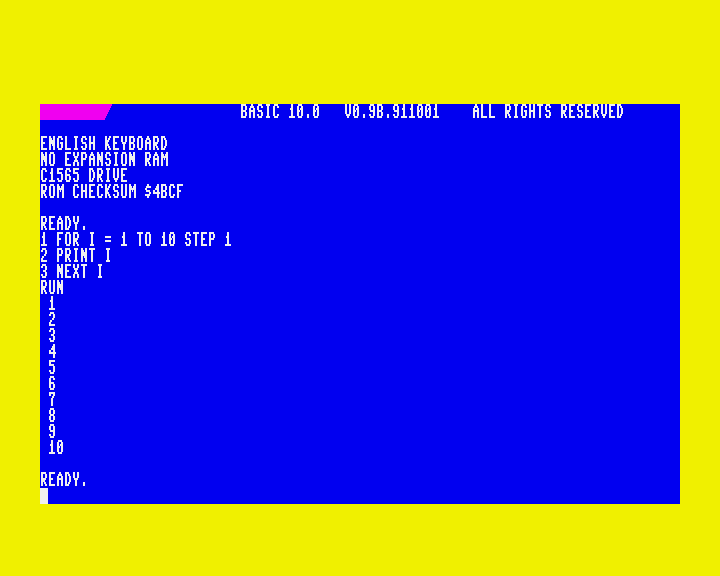
\includegraphics[width=\linewidth]{images/first-steps-for-loop-programme-1-running.png}
  \end{wrapfigure}

  You might notice a couple of things here:

  First, the computer has told us it is \screentext{READY.} again
  as soon as it finished running the programme. This just makes it easier for us to know when we
  can start giving commands to the computer again.

  Second, when the computer got to the bottom of the screen
  it automatically scrolled the display up to make space.  This is quite normal.  What is important
  to remember, is that the computer forgets everything that scrolls off the top.  The only exception
  is if you have told the computer to remember a command by putting a number in front of it.  So
  our programme is quite safe for now. We can see that this is the case by typing the \screentext{RUN} command a
  couple more times: The programme listing will have scrolled off the top of the screen, but we can
  still RUN the programme, because the computer has remembered it.  Give it a try!

  \setlength{\intextsep}{0pt}%
  \begin{wrapfigure}{i}{0.6\linewidth}
    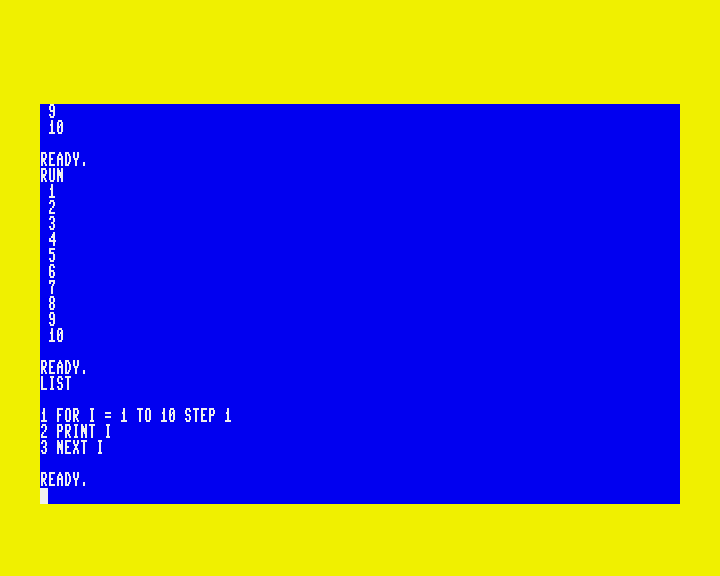
\includegraphics[width=\linewidth]{images/first-steps-for-loop-programme-1-listing.png}
  \end{wrapfigure}

  If you wish to see the programme of remembered commands, you can use the \screentext{LIST}\index{LIST}\index{BASIC 10 Commands!LIST}
  command.  This commands causes the computer to display the remembered programme of commands to the screen, like in the display here.
  If you would like to replace any of the commands in the programme, you can type a new line that has the same number as the one you wish to change. For example, to print the results all on one line, we could modify the second line of the programme to \screentext{PRINT I;} by
  typing the following line of input and pressing the \specialkey{RETURN} key:

\begin{tcolorbox}[colback=black,coltext=white]
\verbatimfont{\codefont}
\begin{verbatim}
2 PRINT I;
\end{verbatim}
\index{PRINT}
\index{BASIC 10 Commands!PRINT}
\end{tcolorbox}

  \setlength{\intextsep}{0pt}%
  \begin{wrapfigure}{i}{0.6\linewidth}
    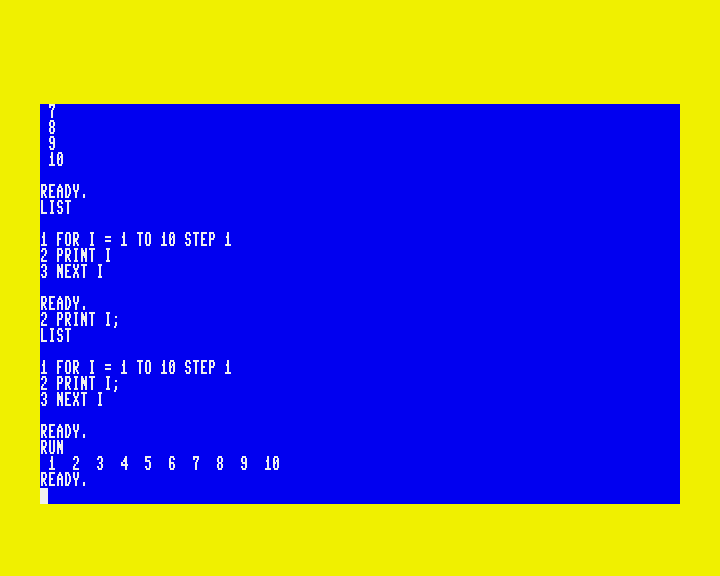
\includegraphics[width=\linewidth]{images/first-steps-for-loop-programme-1-modified.png}
  \end{wrapfigure}

You can make sure that the change has been remembered by running the \screentext{LIST} command again, as we can see here.
You can then use the \screentext{RUN} command to run the modified programme.

It is quite easy to modify your programmes in this way.  As you become more comfortable with the process, there are two
additional helpful tricks:

First, you can give the \screentext{LIST} command the number of a command, or line as they are referred to, and it will display only
that line of the programme.  Alternatively, you can give a range separated by a minus sign to display only a section of the programme,
e.g., \screentext{LIST 1 - 2} to list the first two lines of our programme.

Second, you can use the cursor keys to move the cursor to a line which has already been remembered and is displayed on the screen. If you
modify what you see on the screen, and then press the \specialkey{RETURN} key while the cursor is on that line, the BASIC interpreter will
read in the modified line and replace the old version of it.  It is important to note that if you modify multiple lines of the programme
at the same time, you must press the \specialkey{RETURN} key on each line that has been modified. It is good practice to check that the
programme has been correctly modified. Use the \specialkey{LIST}\index{LIST}\index{BASIC 10 Commands!LIST} command again to achieve this.
  
  
  \subsubsection{Exercises to try}

  {\bf 1. Can you make it count to a higher or lower number?}

  At the moment it counts from 1 to 10.  Can you change it to count to 20 instead?  Or to count from 3 to 17?
  Or how about from 14.5 to 21.5? What do you think you would need to reverse the order in which it counts?

  {\em Clue:} You will need to modify the \screentext{FOR} command.  

  {\bf 2. Can you change the counting step?}

  At the moment it counts by ones, i.e., each number is one more than the last.  Can you change it to count by twos
  instead? Or by halves, so that it counts 1, 1.5, 2, 2.5, 3, \ellipsis?
  
  {\em Clue:} You will need to modify the \screentext{STEP} clause of the \screentext{FOR} command.\index{STEP}\index{BASIC10 Commands!STEP}
  
  
  {\bf 3. Can you make it print out one of the times tables?}
  
  At the moment it prints the answers to the 1 times tables, because it counts by ones.
  Can you make it count by threes, and show the three times tables?
  
  {\em Clue:} You will need to modify the \screentext{FOR} command.
  
  {\bf 4. Can you make it print out the times tables from 1$\times$1 to 10$\times$10?}
  
  {\em Clue:} You might like to use ; on the end of \screentext{PRINT} statements, so that you can have
  more than one entry per line on the screen.\\
  {\em Clue:} The \screentext{PRINT} statement without any argument will just advance to the start of the next line.\\
  {\em Clue:} You might need to have multiple \screentext{FOR} loops, one inside the other.
  
\section{First steps with text and numbers}

\section{Making simple decisions}

\section{Random numbers and chance}
